\documentclass[aspectratio=169,11pt]{beamer}

% ───────────────────────────────────────────────────────────────────────── %
% Tema visual: cremoso + titulo serif navy, similar a "Avance 3".            %
% ───────────────────────────────────────────────────────────────────────── %
\usepackage[utf8]{inputenc}
\usepackage[T1]{fontenc}
\usepackage[spanish,es-tabla]{babel}
\usepackage{lmodern}
\usepackage{amsmath,amssymb}
\usepackage{graphicx}
\usepackage{booktabs}
\usepackage{array}
\usepackage{xcolor}
\usepackage{colortbl}
\usepackage{tikz}
\usepackage{microtype}
\usepackage{pifont}

% Paleta
\definecolor{cream}{HTML}{F2EEE3}
\definecolor{navy}{HTML}{2F3E4E}
\definecolor{accentA}{HTML}{7E57C2}
\definecolor{accentB}{HTML}{EF6C00}
\definecolor{accentC}{HTML}{2E7D32}
\definecolor{accentD}{HTML}{C62828}
\definecolor{rule}{HTML}{B5AFA1}

\setbeamercolor{background canvas}{bg=cream}
\setbeamercolor{normal text}{fg=navy}
\setbeamercolor{frametitle}{fg=navy,bg=cream}
\setbeamercolor{title}{fg=navy}
\setbeamercolor{author}{fg=navy}
\setbeamercolor{structure}{fg=accentC}
\setbeamercolor{itemize item}{fg=accentC}
\setbeamercolor{itemize subitem}{fg=accentB}

\setbeamerfont{frametitle}{family=\rmfamily,series=\bfseries,size=\Large}
\setbeamerfont{title}{family=\rmfamily,series=\bfseries,size=\huge}
\setbeamerfont{subtitle}{family=\rmfamily,size=\large}

\setbeamertemplate{navigation symbols}{}
\setbeamertemplate{frametitle}{%
  \vspace{0.6em}%
  \begin{center}
    \usebeamerfont{frametitle}\usebeamercolor[fg]{frametitle}\insertframetitle
  \end{center}%
  \vspace{-0.4em}%
  {\color{rule}\hrule height 0.6pt}%
  \vspace{0.4em}%
}
\setbeamertemplate{footline}{%
  \hfill\usebeamercolor[fg]{normal text}\small\insertframenumber\hspace{1em}\vspace{0.4em}%
}

% ───────────────────────────────────────────────────────────────────────── %
\title{Sistema de Recomendaci\'on H\'ibrido\\para Pueblos M\'agicos}
\subtitle{An\'alisis de Aspectos y Optimizaci\'on Metaheur\'istica\\
\vspace{0.4em}\textit{Avance de Tesis 4}}
\author{Gustavo Hern\'andez Angeles}
\date{}

\begin{document}

% ───────────────────────────── Portada ─────────────────────────────────── %
\begin{frame}[plain]
	\vspace{1.5em}
	\begin{center}
		{\usebeamerfont{title}\color{navy}Sistema de Recomendaci\'on H\'ibrido\\para Pueblos M\'agicos}\\[0.6em]
		{\usebeamerfont{subtitle}\color{navy}An\'alisis de Aspectos y Optimizaci\'on Metaheur\'istica (?)}\\[0.3em]
		{\color{rule}\rule{0.5\linewidth}{0.4pt}}\\[0.4em]
		{\large\itshape Avance de Tesis 4}
	\end{center}
	\vspace{1.2em}
	\begin{flushleft}
		\textbf{Autor:} Gustavo Hern\'andez Angeles\\
		\textbf{Asesor:} Dr.\ Norberto Alejandro Hern\'andez Leandro\\[0.3em]
		\textbf{Comit\'e de Seguimiento:}\\
		\quad$\bullet$ Dr.\ Alejandro Rosales P\'erez\\
		\quad$\bullet$ Dr.\ Miguel \'Angel \'Alvarez Carmona\\[0.5em]
	\end{flushleft}
\end{frame}

% ───────────────────────────── Objetivos ───────────────────────────────── %
\begin{frame}{Objetivos}
	\small
	\textbf{Objetivo General.}\;
	Elaborar un sistema de recomendaci\'on h\'ibrido (SRH) para Pueblos M\'agicos de M\'exico que integre ABSA, compuesto por modelos colaborativos y basados en contenido, cuyos pesos de fusi\'on se calculen mediante algoritmos de optimizaci\'on.

	\vspace{0.6em}
	\textbf{Objetivos espec\'ificos:}
	\begin{columns}[T]
		\begin{column}{0.5\linewidth}
			\begin{enumerate}\setlength\itemsep{3pt}
				\item[\color{accentC}\ding{51}] Preparar el corpus de trabajo a partir del \textit{dataset} REST-MEX 2025.
				\item[\color{accentC}\ding{51}] Pipeline de ABSA con Zero-Shot y Sentiment Classification.
				\item[\color{accentC}\ding{51}] Derivar las matrices estructurales del sistema (relaci\'on usuarios, \'items, aspectos).
			\end{enumerate}
		\end{column}
		\begin{column}{0.5\linewidth}
			\begin{enumerate}\setlength\itemsep{3pt}
				\item[\color{accentC}\ding{51}] Implementaci\'on de los modelos colaborativos y basados en contenido.
				\item[$\square$] Implementar la fusi\'on de componentes como un problema de optimizaci\'on.
				\item[$\square$] Evaluaci\'on del SRH.
			\end{enumerate}
		\end{column}
	\end{columns}

	\vspace{0.6em}
	\centering
	{\color{rule}\rule{0.4\linewidth}{0.4pt}}\\[0.3em]
	\textit{Avance actual:} \textbf{4/6} objetivos espec\'ificos completados.
\end{frame}

% ───────────────────────────── Recapitulando ───────────────────────────── %
\begin{frame}{Recapitulando...}
	\small
	Desde el \'ultimo avance: pipeline ABSA, matrices estructurales $A,X,Y,R$, y baseline de cuatro modelos con fusi\'on convexa.
	\vspace{0.6em}
	\begin{columns}[T]
		\begin{column}{0.48\linewidth}
			\textbf{Recordatorio - matrices de perfil:}
			\[
				X_{u,j}=1+(N-1)\!\left(\frac{2}{1+e^{-t_{uj}/T_x}}-1\right)
			\]
			\[
				Y_{p,j}=1+\frac{N-1}{1+e^{-k_{pj}\cdot \bar{s}_{pj}/T_y}}
			\]
			$X$: importancia usuario-aspecto.\\
			$Y$: calidad pueblo-aspecto.
		\end{column}
		\begin{column}{0.48\linewidth}
			\textbf{En este avance:}
			\begin{itemize}
				\item \textbf{Ablaci\'on $X/Y$}: explica el efecto del $\log$ y de la $T$.
				\item \textbf{Replanteamiento del h\'ibrido}: pasamos de 4 modelos a un h\'ibrido de \emph{dos} basados en aspectos.
				\item \textbf{Grid-search} sobre un \'unico $\alpha \in [0,1]$.
			\end{itemize}
		\end{column}
	\end{columns}
\end{frame}

% ───────────────────────── Motivacion ablacion ─────────────────────────── %
\begin{frame}{Motivaci\'on del estudio de ablaci\'on}
	\small
	La construcci\'on de $X$ y $Y$ acumul\'o dos modificaciones respecto a Zhang et al.\ (2014):
	\begin{itemize}
		\item En $Y$ se introdujo $\log(1+n)$ para mitigar la saturaci\'on por volumen.
		\item En ambas se a\~nadi\'o un \textbf{t\'ermino de escalamiento} $T$ basado en la mediana, frenando la saturaci\'on temprana del sigmoide.
	\end{itemize}
	\vspace{0.4em}
	\textbf{Pregunta:} ¿cu\'al de estos dos cambios aporta realmente al desempe\~no?\\[0.3em]
	\textbf{Dise\~no:} cuatro variantes cruzadas sobre los modelos que dependen de $X$ y/o $Y$.

	\vspace{0.8em}
	\centering
	\renewcommand{\arraystretch}{1.15}
	\begin{tabular}{c l l}
		\toprule
		\textbf{Variante} & \textbf{$X$}              & \textbf{$Y$}                            \\
		\midrule
		A                 & sigmoide $+\,T$ (actual)  & $h\cdot\log(1+n)+T$ (actual)            \\
		B                 & Zhang Eq.\,2 puro ($T=1$) & Zhang Eq.\,3 puro (sin $\log$, sin $T$) \\
		C                 & Zhang Eq.\,2 puro ($T=1$) & Zhang Eq.\,3 $+\,T$ (sin $\log$)        \\
		D                 & sigmoide $+\,T$ (actual)  & Zhang Eq.\,3 $+\,T$ (sin $\log$)        \\
		\bottomrule
	\end{tabular}
\end{frame}

% ───────────────────── Diagnostico de matrices ─────────────────────────── %
\begin{frame}{Diagn\'ostico de las matrices}
	\small
	Antes de evaluar ranking: ¿c\'omo se ven $X$ y $Y$ en cada variante?
	\vspace{0.4em}
	\centering
	\renewcommand{\arraystretch}{1.12}
	\begin{tabular}{c c c c c c c}
		\toprule
		\textbf{Var.}  & $\overline{X}$                  & $\mathrm{Var}_{\text{fila}}(X)$ & $X{>}4.5$ &
		$\overline{Y}$ & $\mathrm{Var}_{\text{fila}}(Y)$ & $Y{>}4.5$                                                                   \\
		\midrule
		A              & 2.31                            & 1.00                            & 9.6\%     & 3.90 & 0.09 & 1.3\%           \\
		B              & 3.09                            & 1.88                            & 36.5\%    & 4.94 & 0.15 & \textbf{97.9\%} \\
		C              & 3.09                            & 1.88                            & 36.5\%    & 4.04 & 0.23 & 33.6\%          \\
		D              & 2.31                            & 1.00                            & 9.6\%     & 4.04 & 0.23 & 33.6\%          \\
		\bottomrule
	\end{tabular}
	\vspace{0.6em}

	\begin{columns}[T]
		\begin{column}{0.5\linewidth}
			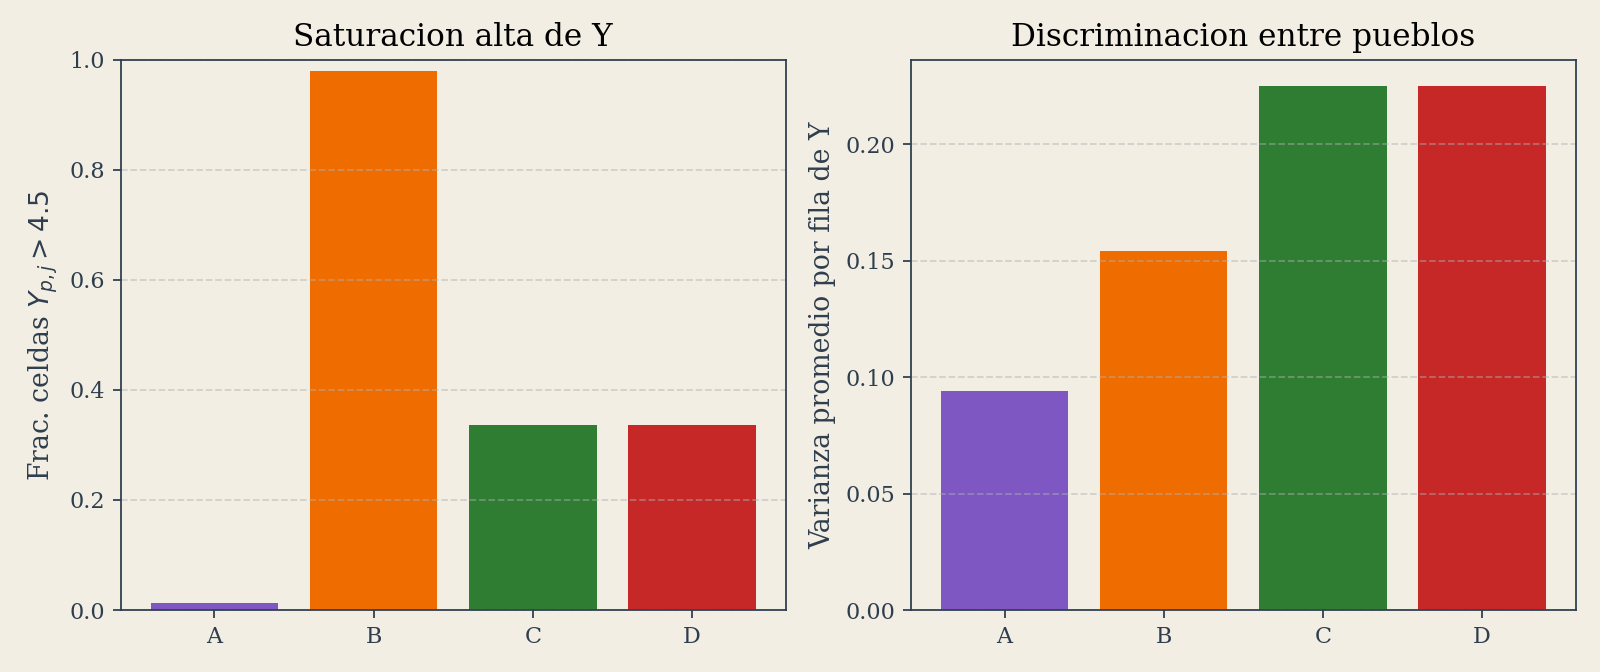
\includegraphics[width=\linewidth]{figures/y_diagnostics.png}
		\end{column}
		\begin{column}{0.46\linewidth}
			\textbf{Lectura:}
			\begin{itemize}\setlength\itemsep{2pt}
				\item En \textbf{B}, $Y$ colapsa: 97.9\% de celdas $>4.5$.
				\item $T$ (C, D) recupera varianza por fila ($0.23$ vs $0.15$).
				\item $\log(1+n)$ (A) degrada la se\~nal: $\overline{Y}=3.90$.
			\end{itemize}
		\end{column}
	\end{columns}
\end{frame}

% ───────────────────────── Resultados K=10 ─────────────────────────────── %
\begin{frame}{Resultados de ablaci\'on \;|\; $K=10$}
	\centering
	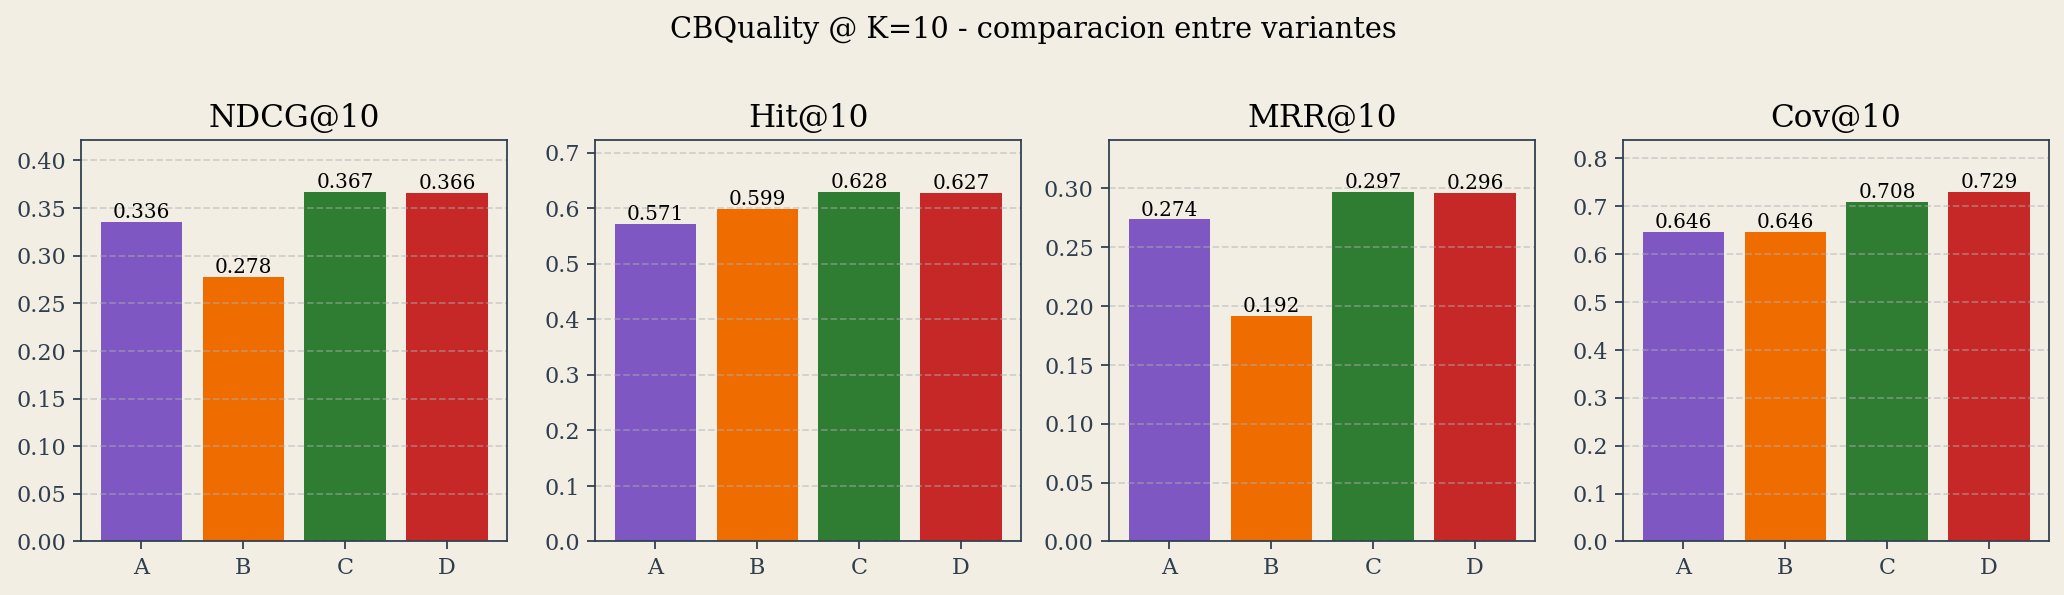
\includegraphics[width=0.97\linewidth]{figures/summary_k10.png}
	\vspace{-0.2em}
	\small

	\begin{itemize}\setlength\itemsep{2pt}
		\item \textbf{CBQuality} domina ranking: $\mathbf{C}$ alcanza $\text{NDCG@10}=0.3666$ (vs.\ A: 0.3358, B: 0.2778, D: 0.3658).
		\item Cobertura@10 mejora $\sim 8$ puntos pasando de A a C/D.
		\item El \emph{quitar} $\log(1+n)$ pero \emph{conservar} $T$ (C, D) es la mejor combinaci\'on.
	\end{itemize}
\end{frame}

% ───────────────────── NDCG por K para CBQuality ───────────────────────── %
\begin{frame}{CBQuality \;|\; NDCG@K y Cobertura@K}
	\begin{columns}[c]
		\begin{column}{0.5\linewidth}
			\centering
			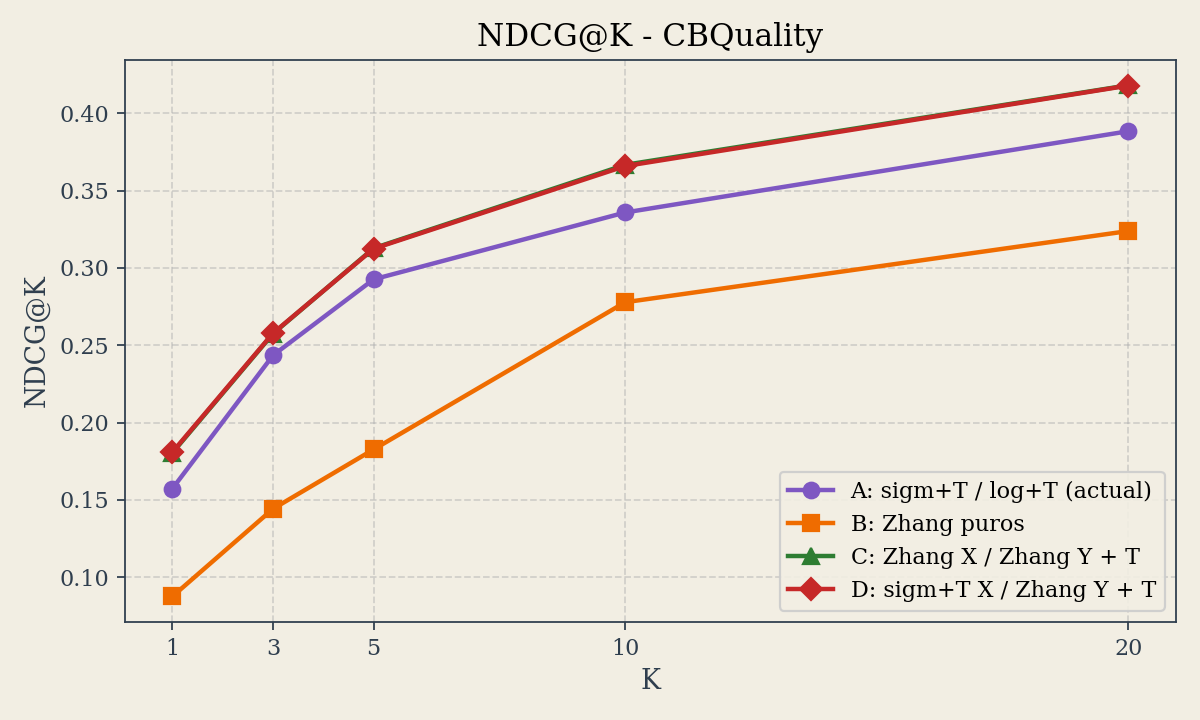
\includegraphics[width=\linewidth]{figures/ndcg_cbquality.png}
		\end{column}
		\begin{column}{0.5\linewidth}
			\centering
			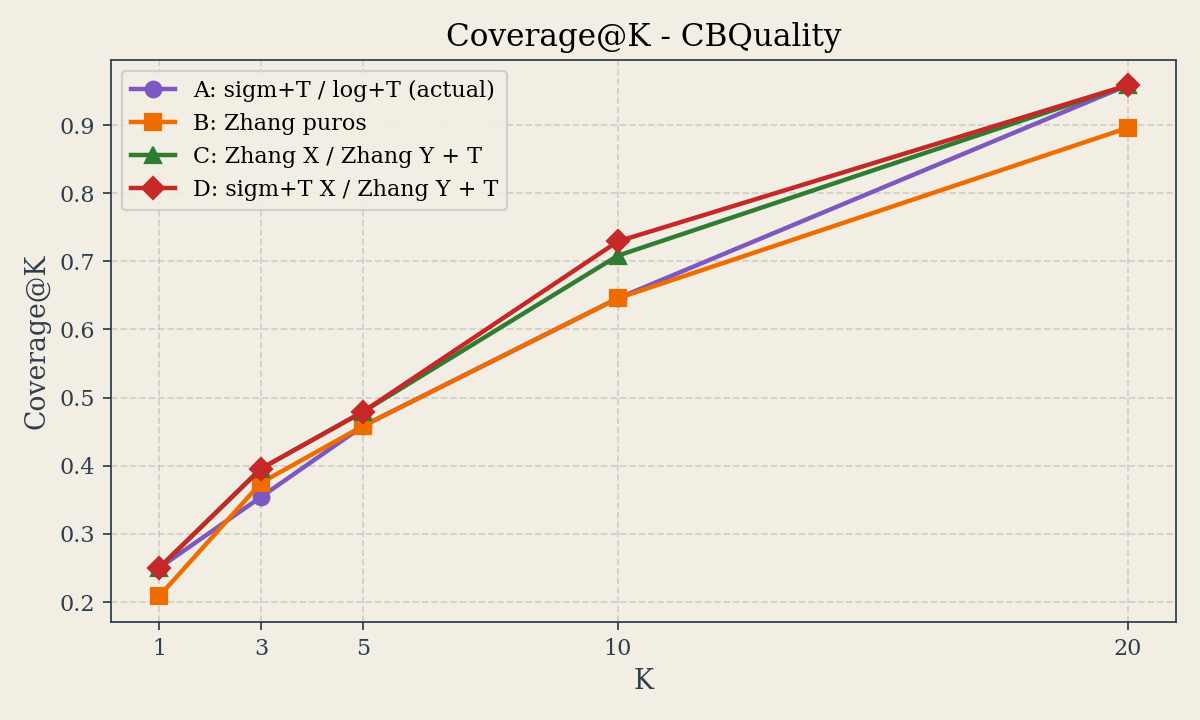
\includegraphics[width=\linewidth]{figures/cov_cbquality.png}
		\end{column}
	\end{columns}
	\vspace{0.4em}
	\small
	Las curvas $C$ y $D$ son \emph{indistinguibles} en ranking pero D mantiene una cobertura ligeramente superior $(0.7292$ vs $0.7083$ @ $K=10)$.
\end{frame}

% ─────────────── NDCG por K para CBAttention (sanity check) ─────────────── %
\begin{frame}{CF Atencion \;|\; insensibilidad a $Y$}
	\begin{columns}[c]
		\begin{column}{0.55\linewidth}
			\centering
			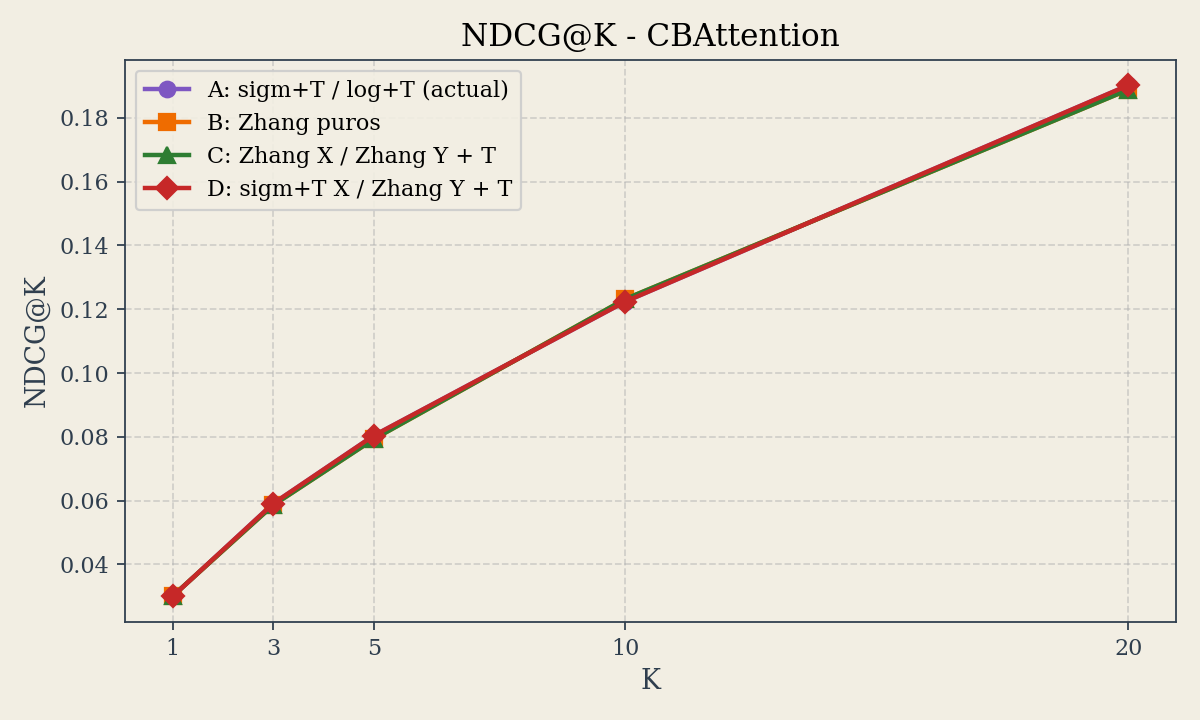
\includegraphics[width=\linewidth]{figures/ndcg_cbattention.png}
		\end{column}
		\begin{column}{0.45\linewidth}
			\small
			\textbf{Sanity check:} {\tt CFAttention} s\'olo usa $X$.
			\begin{itemize}\setlength\itemsep{3pt}
				\item Variantes con la misma $X$ producen NDCG id\'enticos:
				      \[
					      \text{A}\!=\!\text{D},\quad \text{B}\!=\!\text{C}.
				      \]
				\item Confirma que la implementaci\'on es correcta y que las diferencias en {\tt CBQuality} provienen de $Y$, no del azar.
			\end{itemize}
		\end{column}
	\end{columns}
\end{frame}

% ───────────────────── Conclusion ablacion ─────────────────────────────── %
\begin{frame}{Conclusiones del estudio de ablaci\'on}
	\small
	\begin{itemize}\setlength\itemsep{4pt}
		\item El cuello de botella estaba en $Y$: la Eq.\,3 de Zhang \textbf{satura} (97.9\% de celdas en $\!>\!4.5$).
		\item El \textbf{t\'ermino de escalamiento} $T$ basado en la mediana es la \emph{contribuci\'on dominante}: por s\'i solo recupera la discriminaci\'on entre pueblos.
		\item El $\log(1+n)$ resultaba redundante (y sub-\'optimo) cuando ya hay $T$.
	\end{itemize}

	\vspace{0.6em}
	\centering
	\renewcommand{\arraystretch}{1.1}
	\begin{tabular}{c c c c c}
		\toprule
		\textbf{Var.} & NDCG@10         & Cov@10          & MRR@10          & Hit@10          \\
		\midrule
		A             & 0.3358          & 0.6458          & 0.2736          & 0.5714          \\
		B             & 0.2778          & 0.6458          & 0.1918          & 0.5988          \\
		\rowcolor{cream!50}
		C             & \textbf{0.3666} & 0.7083          & \textbf{0.2967} & \textbf{0.6285} \\
		\rowcolor{cream!50}
		D             & 0.3658          & \textbf{0.7292} & 0.2962          & 0.6269          \\
		\bottomrule
	\end{tabular}

	\vspace{0.5em}
	\textbf{Decisi\'on:} adoptar la variante \textbf{D} ($X$ sigmoide$+T$, $Y$ Zhang $+T$) como construcci\'on canon.
\end{frame}

% ─────────────────────── Replanteamiento ───────────────────────────────── %
\begin{frame}{Replanteamiento del h\'ibrido}
	\small
	\textbf{Antes:} cuatro modelos en combinaci\'on convexa,
	$\hat y_{u,p}(\mathbf{w}) = \sum_{m=1}^{4} w_m \,\hat y^{(m)}_{u,p}$, con $\mathbf{w}\in\Delta^{3}$.

	\vspace{0.4em}
	\textbf{Hallazgos de la evaluaci\'on previa (Avance 3):}
	\begin{itemize}\setlength\itemsep{2pt}
		\item {\tt CBQuality} domina las m\'etricas de \textbf{ranking} (NDCG, MRR, Hit).
		\item {\tt CFAttention} domina la \textbf{cobertura} del cat\'alogo.
	\end{itemize}

	\vspace{0.5em}
	\textbf{Propuesta:} h\'ibrido de \emph{dos} modelos, ambos basados en se\~nales ABSA (aspectos $+$ sentimiento):
	\[
		\boxed{\;\hat y_{u,p}(\alpha) \;=\; \alpha\,\hat y^{\mathtt{CBAttention}}_{u,p} \;+\; (1-\alpha)\,\hat y^{\mathtt{CBQuality}}_{u,p}\;}
	\]
	\textbf{Ventajas:}
	\begin{itemize}\setlength\itemsep{2pt}
		\item Refuerza la contribuci\'on metodol\'ogica: la fusi\'on se hace entre dos sub-sistemas que \emph{consumen ABSA}.
		\item Espacio de b\'usqueda 1D $\Rightarrow$ \textbf{grid-search} en $\alpha$ basta; no se necesita PSO/DE/BO.
	\end{itemize}
\end{frame}

% ─────────────────────── Formulacion ──────────────────────────────────── %
\begin{frame}{Formulaci\'on de la b\'usqueda en $\alpha$}
	\small
	Sea $\hat y^{(m)}_{u,p}$ el score normalizado del modelo $m$. Definimos
	\[
		\hat y_{u,p}(\alpha) \;=\; \alpha\,\hat y^{\mathtt{CFAttention}}_{u,p} \;+\; (1-\alpha)\,\hat y^{\mathtt{CBQuality}}_{u,p},
		\qquad \alpha \in [0,1].
	\]
	La funci\'on objetivo agrega ranking y diversidad:
	\[
		f(\alpha)\;=\;\beta\,\mathrm{NDCG@K}(\alpha)\;+\;(1-\beta)\,\mathrm{Cov@K}(\alpha),
		\qquad
		\alpha^{\!*} \in \arg\max_{\alpha\in[0,1]} f(\alpha).
	\]

	\textbf{Implementaci\'on:}
	\begin{itemize}\setlength\itemsep{2pt}
		\item Una sola pasada: se ajustan {\tt CFAttention} y {\tt CBQuality} y se precomputan los scores.
		\item Por cada $\alpha$ de la grilla ($\alpha\!\in\!\{0, 0.05, \dots, 1\}$ por defecto), s\'olo se ponderan los scores.
	\end{itemize}
\end{frame}

% ─────────────────────── Pipeline grafico ──────────────────────────────── %
\begin{frame}{Pipeline del nuevo h\'ibrido}
	\centering
	\begin{tikzpicture}[
			every node/.style={font=\small, color=navy},
			box/.style={draw=navy, fill=cream, rounded corners, thick, minimum width=2.5cm, minimum height=0.9cm, align=center},
			arr/.style={-latex, thick, draw=accentC},
			matrix/.style={draw=accentB, fill=cream, rounded corners, thick, minimum width=1.4cm, minimum height=0.8cm, align=center}
		]
		\node[matrix] (A) at (-5,0) {$A$\\\tiny ratings};
		\node[matrix] (X) at (-5,-1.4) {$X$\\\tiny importancia};
		\node[matrix] (Y) at (-5,-2.8) {$Y$\\\tiny calidad};

		\node[box] (cba) at (-1.0, -0.3) {\tt CBAttention\\$\hat y^{(\text{att})}$};
		\node[box] (cbq) at (-1.0, -2.5) {\tt CBQuality\\$\hat y^{(\text{qual})}$};

		\node[box, fill=accentC!20] (hyb) at (3.5, -1.4) {Fusi\'on\\$\alpha\,\hat y^{(\text{att})} + (1-\alpha)\hat y^{(\text{qual})}$};

		\node[box, fill=accentB!20] (grid) at (8.0, -1.4) {\textbf{Grid-search}\\sobre $\alpha\in[0,1]$\\m\'ax $f(\alpha)$};

		\draw[arr] (X) -- (cba.west);
		\draw[arr] (A) -- (cba.west);
		\draw[arr] (X) -- (cbq.west);
		\draw[arr] (Y) -- (cbq.west);
		\draw[arr] (cba.east) -- (hyb.west);
		\draw[arr] (cbq.east) -- (hyb.west);
		\draw[arr] (hyb.east) -- (grid.west);
	\end{tikzpicture}
	\vspace{0.6em}

	\small
	Ambos sub-sistemas se entrenan una sola vez. El barrido en $\alpha$ es \emph{barato}: s\'olo cambia un escalar.
\end{frame}

% ─────────────────────── Pr\'oximos pasos ──────────────────────────────── %
\begin{frame}{Pr\'oximos pasos}
	\small
	\begin{enumerate}\setlength\itemsep{4pt}
		\item Ejecutar el barrido $\alpha\in\{0,0.05,\dots,1\}$ y reportar la curva NDCG/Cov vs.\ $\alpha$.
		\item Decidir $\alpha^{*}$ por criterio multi-objetivo (Pareto NDCG-Coverage) o por $\beta$ fijo.
		\item Cerrar redacci\'on de Cap\'itulo 4 (resultados) e iniciar correcciones para defensa.
	\end{enumerate}

	\vspace{0.8em}
	\centering
	{\color{rule}\rule{0.5\linewidth}{0.4pt}}\\[0.5em]
	\textit{Objetivos espec\'ificos del proyecto:} \textbf{4/6 completados}.\\
	\textit{Resta:} fijar $\alpha^{*}$ (Obj.\ 5) y evaluaci\'on final del SRH (Obj.\ 6).
\end{frame}

% ─────────────────────── Gracias ───────────────────────────────────────── %
\begin{frame}[plain]
	\vfill
	\begin{center}
		{\fontsize{60}{72}\selectfont\bfseries\rmfamily\color{navy}GRACIAS}
	\end{center}
	\vfill
\end{frame}

\end{document}
